\documentclass[12pt]{article}
\usepackage[pdftex]{graphicx}
\newcommand{\kg}{\mathrm{kg}}
\newcommand{\m}{\mathrm{m}}
\newcommand{\cm}{\mathrm{cm}}
\newcommand{\mi}{\mathrm{mi}}
\newcommand{\s}{\mathrm{s}}
\newcommand{\ms}{\mathrm{ms}}
\newcommand{\h}{\mathrm{h}}
\newcommand{\N}{\mathrm{N}}
\newcommand{\W}{\mathrm{W}}
\newcommand{\hp}{\mathrm{hp}}
\newcounter{problem}
\stepcounter{problem}
\newcounter{answer}[problem]
\newenvironment{problem}{\noindent\begin{minipage}{\textwidth}\sloppy\sloppypar\raggedright\textbf{\theproblem.}\refstepcounter{problem}\stepcounter{answer}---}{\end{minipage}\vspace{2ex}}
\newcommand{\source}[1]{[{#1}]}
\newenvironment{answers}{\\}{}
\newcommand{\answer}[1]{\textbf{\Alph{answer}:}\refstepcounter{answer}~\mbox{#1}\hspace{3ex}}
\begin{document}

\section*{NYU General Physics 1---Term Exam 2}

\begin{problem}
  \source{from lecture 2011-10-06} I swung a coffee cup over my head
  and the coffee did not spill out.  If, at the top of the swing, the
  cup was moving at speed $v$ on a circular path of radius $R$, what
  needed to be true for the coffee to stay securely in the cup?
  \begin{answers}
    \answer{$\displaystyle \frac{v^2}{R} = 0$}
    \answer{$\displaystyle \frac{v^2}{R} < g$}
    \answer{$\displaystyle \frac{v^2}{R} = g$}
    \answer{$\displaystyle \frac{v^2}{R} > g$}
    \answer{None of these}
  \end{answers}
\end{problem}

\begin{problem}
  \source{from lecture 2011-10-13} We considered a block sliding down
  a frictionless hill and off a frictionless jump.  The block flew up
  into the air, but it did not return to the height from which it
  started.  Why not?
  \begin{answers}
    \answer{Energy was not conserved.}
    \answer{The block lost energy to heat during its slide.}
    \answer{Not all of the potential energy was converted into kinetic energy.}
    \answer{After the jump, the horizontal component of velocity is constant.}
    \answer{There are energies other than kinetic and potential to consider.}
  \end{answers}
\end{problem}

\begin{problem}
  \source{from lecture 2011-10-18} A small bullet of mass $m$ moving
  at velocity $\vec{v}$ lodged in a big block of mass $M$.
  Immediately before the collision, the bullet had momentum $\vec{p}_i =
  m\,\vec{v}$ and kinetic energy $K_i = (1/2)\,m\,|\vec{v}|^2$.
  Immediately after the collision, the momentum $\vec{p}_f$ and kinetic
  energy $K_f$ of the bullet+block system were
  \begin{answers}
    \answer{$|\vec{p}_f| = |\vec{p}_i|$ and $K_f = K_i$}
    \answer{$|\vec{p}_f| = |\vec{p}_i|$ and $K_f < K_i$}
    \answer{$|\vec{p}_f| = |\vec{p}_i|$ and $K_f > K_i$}
    \answer{$|\vec{p}_f| < |\vec{p}_i|$ and $K_f = K_i$}
    \answer{$|\vec{p}_f| > |\vec{p}_i|$ and $K_f = K_i$}
  \end{answers}
\end{problem}

\begin{problem}
  \source{from lecture 2011-10-18} A block of mass $[M+m]$ attached to
  the ceiling by a string of length $L$ is moving at speed $v_f$ when
  the string is vertical, that is, when the block is at the minimum of
  potential energy.  It will then swing up to some maximum height
  $h_\mathrm{max}$ given by
  \begin{answers}
    \answer{$\displaystyle h_\mathrm{max} = \frac{v_f}{2\,g}$}
    \answer{$\displaystyle h_\mathrm{max} = \frac{v_f^2}{g}$}
    \answer{$\displaystyle h_\mathrm{max} = \frac{v_f}{g}$}
    \answer{$\displaystyle h_\mathrm{max} = \frac{v_f^2}{2\,g}$}
    \answer{none of these}
  \end{answers}
\end{problem}

\begin{problem}
  \source{from lecture 2011-10-20} A block of mass $5.0\,\kg$ moves at
  $2.0\,\m\,\s^{-1}$ in the positive $x$ direction and a block of mass
  $3.0\,\kg$ moves at $3.0\,\m\,\s^{-1}$ in the negative $x$
  direction.  What is the $x$-direction velocity of the center of mass
  (or the velocity of the center-of-mass frame)?
  \begin{answers}
    \answer{$\displaystyle 0.125\,\m\,\s^{-1}$}
    \answer{$\displaystyle 0.5\,\m\,\s^{-1}$}
    \answer{$\displaystyle 1.0\,\m\,\s^{-1}$}
    \answer{$\displaystyle 2.375\,\m\,\s^{-1}$}
    \answer{$\displaystyle 19.0\,\m\,\s^{-1}$}
  \end{answers}
\end{problem}

\begin{problem}
  \source{from lecture 2011-10-25} We found the forces on a light
  table holding a very heavy block of mass $M$.  The table was
  supported by two supports (support 1 and support 2) separated by a
  distance $L$.  The block was a distance $x$ from support 1.  The
  ratio of the normal force $N_2$ at support 2 to the normal force
  $N_1$ at support 1 was
  \begin{answers}
    \answer{$\displaystyle \frac{N_2}{N_1} = \left|x\right|$}
    \answer{$\displaystyle \frac{N_2}{N_1} = \left|x - L\right|$}
    \answer{$\displaystyle \frac{N_2}{N_1} = \left|\frac{x}{x - L}\right|$}
    \answer{$\displaystyle \frac{N_2}{N_1} = \left|\frac{x - L}{x}\right|$}
    \answer{none of these}
  \end{answers}
\end{problem}

\begin{problem}
  \source{from lecture 2011-10-27} The hanging sign problem we did had
  a cable that made an angle $\theta$ with respect to the horizontal
  direction.  Imagine making $\theta$ very small, so the cable is
  nearly horizontal.  What happens to the tension $T$ in the cable as
  $\theta$ gets small?
  \begin{answers}
    \answer{$T$ gets very small}
    \answer{$T$ approaches $M\,g + m\,g/2$}
    \answer{$T$ gets very large}
    \answer{$T$ doesn't depend on $\theta$}
    \answer{none of these}
  \end{answers}
\end{problem}

\begin{problem}
  \source{from lecture 2011-11-01} Stress is proportional to strain.
  What formula is most related to this fact?
  \begin{answers}
    \answer{$\displaystyle \vec{F} = m\,\vec{a}$}
    \answer{$\displaystyle \vec{F} = -k\,\vec{x}$}
    \answer{$\displaystyle E = \frac{1}{2}\,m\,v^2$}
    \answer{$\displaystyle E = \frac{|\vec{p}|^2}{2\,m}$}
    \answer{$\displaystyle \vec{p} = m\,\vec{v}$}
  \end{answers}
\end{problem}

\begin{problem}
  \source{from problem set 5, problem 1} The driver of a car traveling
  east slams on the brakes, so that the car goes through a period of
  rapid deceleration.  The total force on the ground from the car must
  \begin{answers}
    \answer{have a downwards component and an eastwards component}
    \answer{have a downwards component and a westward component}
    \answer{have an upwards component and an eastwards component}
    \answer{have an upwards component and a westward component}
  \end{answers}
\end{problem}

\begin{problem}
  \source{from problem set 5, problem 1} You are sitting in the
  passenger seat of a car moving forwards at high speed but also
  rapidly decelerating, with your seatbelt securely fastened.  The
  deceleration has been going on for some time, and you are tightly
  held in your seat by your seatbelt.  What is the direction of the
  net force acting on you?
  \begin{answers}
    \answer{There is (almost) no net force acting on you.}
    \answer{The net force points towards the front of the car.}
    \answer{The net force points towards the back of the car.}
    \answer{The net force points downwards.}
  \end{answers}
\end{problem}

\begin{problem}
  \source{from problem set 5, problem 2} Why do the astronauts in the
  Space Station feel weightless?
  \begin{answers}
    \answer{There is no gravity in space.}
    \answer{The Space Station is accelerating downwards at $\vec{g}$.}
    \answer{The Space Station is going on a circular trajectory.}
    \answer{The Space Station is very far from Earth.}
  \end{answers}
\end{problem}

\begin{problem}
  \source{from problem set 5, problem 3} You may have learned
  something like $P\,V = n\,R\,T$, where $P$ is pressure (force per
  area) and $V$ is volume.  Whether or not you ever have heard that,
  what are the units of this equation?  Note: You don't need to know
  what $n$, $R$, or $T$ are to solve this problem.
  \begin{answers}
    \answer{force}
    \answer{energy}
    \answer{mass}
    \answer{length}
    \answer{momentum}
  \end{answers}
\end{problem}

\begin{problem}
  \source{from problem set 6, problem 1} You computed the energy
  expended by a college-age human by considering the potential energy
  gain over time of climbing 9 flights of stairs at a reasonable pace.
  The human also has kinetic energy during this climb.  Compare the
  kinetic energy $K$ of the human during the climb to her or his total
  change in potential energy $\Delta U$ during the climb.
  \begin{answers}
    \answer{$K$ is much less than $\Delta U$.}
    \answer{$K$ is about equal to $\Delta U$.}
    \answer{$K$ is much greater than $\Delta U$.}
    \answer{It is impossible to answer this question.}
  \end{answers}
\end{problem}

\begin{problem}
  \source{from problem set 6, problem 1} A good athelete can climb
  stairs at a mechanical energy output of $1\,\hp$ (horesepower).
  Roughly how long would it take such an athelete to climb nine
  flights of stairs?
  \begin{answers}
    \answer{$0.03\,\s$}
    \answer{$0.3\,\s$}
    \answer{$3\,\s$}
    \answer{$30\,\s$}
    \answer{$300\,\s$}
  \end{answers}
\end{problem}

\begin{problem}
  \source{from problem set 6, problem 2} If you compare the energy
  content of gasoline and olive oil, you find that
  \begin{answers}
    \answer{olive oil has more than 10 times higher energy density}
    \answer{they are about the same}
    \answer{gasoline has more than 10 times higher energy density}
  \end{answers}
\end{problem}

\begin{problem}
  \source{from problem set 6, problem 3} A ball bounces on a hard
  surface.  In the period between bounces, when the ball is in
  free-fall, a graph of the kinetic energy as a function of time will
  look like
  \begin{answers}
    \answer{a straight line}
    \answer{two straight lines connected at a point}
    \answer{a parabola going from high to low to high}
    \answer{a parabola going from low to high to low}
    \answer{none of these}
  \end{answers}
\end{problem}

\begin{problem}
  \source{from problem set 7, problem 1} Which of these figures---cut
  from a sheet of constant-thickness aluminum---has its center of
  mass \emph{precisely} at the point $(0,0)$?
  \begin{answers}
  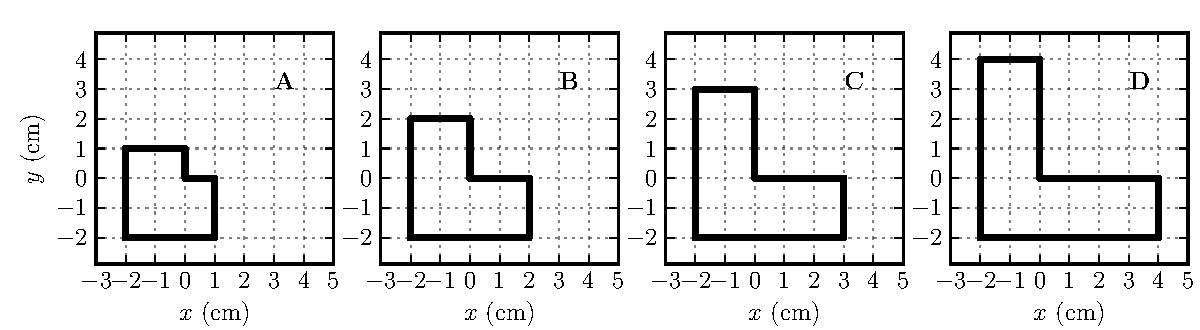
\includegraphics[width=\textwidth]{../py/com_shapes.pdf}\addtocounter{answer}{4}
  \answer{none of these}
  \end{answers}
\end{problem}

\begin{problem}
  \source{from problem set 7, problem 2} Just before jumping out of
  the way, a (daring) student throws a ball at $10\,\mi\,\h^{-1}$
  straight at a bus moving towards the student at $35\,\mi\,\h^{-1}$.
  Assume that these are the speeds just before the collision, that the
  collision is head-on, that the collision is elastic, and that the
  front of the bus is a flat, vertical plane.  Right after the
  collision (after the ball leaves contact with the bus), what will be
  the speed of the ball?  Give your answer for the original reference
  frame.
  \begin{answers}
    \answer{$60\,\mi\,\h^{-1}$}
    \answer{$70\,\mi\,\h^{-1}$}
    \answer{$80\,\mi\,\h^{-1}$}
    \answer{$90\,\mi\,\h^{-1}$}
  \end{answers}
\end{problem}

\begin{problem}
  \source{from problem set 7, problem 3} A student of mass
  $m_\mathrm{student} = 80\,\kg$ stands at rest next to a block of ice
  of mass $m_\mathrm{ice} = 160\,\kg$, also at rest, on a frictionless
  frozen lake.  The student pushes on the block until both the student
  and the block are moving (in opposite directions).  What is the
  ratio of their speeds?
  \begin{answers}
    \answer{$\displaystyle\frac{|\vec{v}_\mathrm{student}|}{|\vec{v}_\mathrm{ice}|} = 4$}
    \answer{$\displaystyle\frac{|\vec{v}_\mathrm{student}|}{|\vec{v}_\mathrm{ice}|} = 2$}
    \answer{$\displaystyle\frac{|\vec{v}_\mathrm{student}|}{|\vec{v}_\mathrm{ice}|} = \sqrt{2}$}
    \answer{$\displaystyle\frac{|\vec{v}_\mathrm{student}|}{|\vec{v}_\mathrm{ice}|} = 1$}
    \answer{$\displaystyle\frac{|\vec{v}_\mathrm{student}|}{|\vec{v}_\mathrm{ice}|} = \frac{1}{2}$}
  \end{answers}
\end{problem}

\begin{problem}
  \source{from problem set 8, problem 1} In this bridge, is the very
  top strut (across the top) in compression or tension?\\
  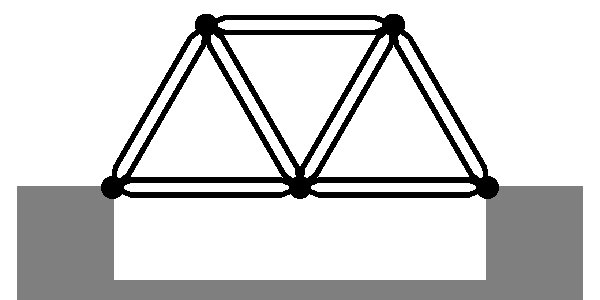
\includegraphics{../py/bridge.pdf}
  \begin{answers}
    \answer{compression}
    \answer{tension}
    \answer{neither}
    \answer{depends}
  \end{answers}
\end{problem}

\begin{problem}
  \source{from problem set 8, problem 2} When you are holding a heavy
  bag of weight $N$ (heavier than your arm) in your arm, and you have
  your arm angled so the upper arm is vertical and the forearm is
  horizontal, there is a tension force $T$ in your bicep muscle and a
  compression force $F_h$ in your humerus bone (the vertical bone in
  your upper arm).  In addition to gravity, these three forces ($N$,
  $T$, and $F_h$) are all acting on the lower part of the arm.
  \begin{answers}
    \answer{$|F_h|>|N|>|T|$}
    \answer{$|N|>|F_h|>|T|$}
    \answer{$|F_h|>|T|>|N|$}
    \answer{$|T|>|N|>|F_h|$}
    \answer{$|T|>|F_h|>|N|$}
  \end{answers}
\end{problem}

\begin{problem}
  \source{from problem set 8, problem 3} A ladder leans in static
  equilibrium against a frictionless wall, making an angle $\theta$
  with the vertical.  How does the normal force $N$ between the floor
  and the ladder vary as we increase $\theta$ (make the ladder less
  vertical)?
  \begin{answers}
    \answer{$N$ increases}
    \answer{$N$ decreases}
    \answer{$N$ stays the same}
  \end{answers}
\end{problem}

\begin{problem}
  \source{from \textit{Newton's Second Law} lab} In one of the
  experiments, a glider mass is attached to a hanging mass by a string
  going over a pulley.  In the theory for this experiment, you assumed
  that the ``smart pulley'' was massless.  This assumption was made to
  \begin{answers}
    \answer{ensure that Newton's law holds}
    \answer{make sure the smart pulley reads out correct information}
    \answer{reduce the friction in the system}
    \answer{make the tension in the string single-valued}
  \end{answers}
\end{problem}

\begin{problem}
  \source{from \textit{Centripetal Force} lab} What is the
  relationship between the angular frequency $\omega$ and the period
  $T$?
  \begin{answers}
    \answer{$\displaystyle\omega = \frac{2\pi}{T}$}
    \answer{$\displaystyle\omega = \frac{T}{2\pi}$}
    \answer{$\displaystyle\omega = 2\pi\,T$}
    \answer{$\displaystyle\omega = \frac{1}{2\pi\,T}$}
    \answer{you need more information to answer this}
  \end{answers}
\end{problem}

\begin{problem}
  \source{from \textit{Conservation of Energy} lab} The spring used in
  this lab had a spring constant $k$ with units of $N\,m^{-1}$, and a
  mass $m$ attached to it.  If you compress the spring by a distance
  $x$, you store potential energy $U$, where
  \begin{answers}
    \answer{$U = m\,k\,x$}
    \answer{$U = (1/2)\,m\,k\,x^2$}
    \answer{$U = (1/2)\,k\,x^2$}
    \answer{$U = (1/3)\,k\,x^3$}
    \answer{$U = \sqrt{k/m}$}
  \end{answers}
\end{problem}

\end{document}
